\chapter{Statistical Model}
\label{chap:statistical_model}

\lettrine{I}{ntroduction} into this chapter\dots

\pagebreak

\section{Time series analysis}
\label{sec:time_series_analysis}

\section{Regression and classification with Gaussian processes}
\label{sec:gaussian_processes}

\todo[inline]{introduction to GP. search over all functions. emphasize the aspects of it that we are using it for, but also a bit generally why it's good for ML. compare it to other interpolation/extrapolation methods. if makes sense, explain to what kind of data it suits.}

%\subsection{Covariance functions (kernels)}
\subsection{Kernel building and tuning}
\label{subsec:covariance_functions}

\todo[inline]{current information taken from \url{http://scikit-learn.org/stable/modules/gaussian_process.html}. in the introduction add the reference(s) mention at the end of this page.}
\todo[inline]{also, there was a very detailed thesis/paper about kernels, check if there are more good details there}

Kernels (also called \textit{Covariance functions} in the context of \acp{gp}) are a key component \acp{gp}, as they define the statistical relationship between the input values.
In general, they represent describe the similarity $k(x, x')$ between each pair of input points, so that $k(\cdot, \cdot)$ determines how similar the outputs $y_*$ and $y_*'$ will be. 
More formally, a covariance function can be described as $\mathcal{K}(x, x') = \phi(x) \cdot \phi(x')$, where $\phi(\cdot)$ is a function that maps the input vectors into a transformed feature space.
Which function to use is a key question when modeling using a \ac{gp}, as it determines the behavior of the model and the quality of the predictions it will be able to make.
Naturally, some assumptions and decisions regarding the data must be made when choosing a kernel.
A kernel's parameters are optimized to achieve functions that better fit the data, the consistency of the resulted functions is measured using log maximum likelihood.

Since convergence analyses usually refer to the \textit{difference} between values in different production (as opposed to the values themselves), stationary kernels are more suitable for fitting \ac{gp} to them, as they are shaped by the distances between each pair of data point rather than their absolute values.
%That is, they fulfill $k(x_1, x_2) = k(x_1 - x_2)$.
%This list only covers a small subset of common covariance functions.
%Further kernels include the exp-sine squared, dot-product, linear, and more.
%\putref{put 2 references about kernels, or only 1 is the first is used above}
Kernels can also be chained using multiplication or addition to combine characteristics of multiple kernels.
Multiplication-based kernels are maximized when all of its kernel factors yield high values, whereas
Addition-based kernels, are maximized when any of their addend kernels yield a high value.
%For example, multiplying a linear kernel by a periodic one will result in functions that are \textit{both} periodic \textit{and} with increasing amplitude as they move away from the origin.
For the modeling presented here, an additive kernel is used with constant, RBF, and noise terms (see \crefrange{eq:constant_kernel}{eq:RBF_kernel}).
The RBF term determines the general shape of the curve (see example in \cref{fig:RBF_prior_posterior}), the constant term enables shifting of the curve if necessary, and the noise term adds degrees of freedom in case the curve cannot completely fit the input signal.

The definitions of the used kernels are as follows:

\begin{description}
	
	\item[Constant kernel -- ]
	This is a simple kernel that assigns the same value for all input pairs.
	Since by itself it does not offer a lot of characteristic to the covariance function, it is usually used as part of a product kernel, where which it scales the magnitude of the other factors, or as part of a sum kernel, in which it modifies the mean of the Gaussian process.
	It has a single parameter, the constant value, and it is defined as 
	%
	\begin{equation}
		\label{eq:constant_kernel}
		k_{constant}(C, x, x') = C\forall x_1, x_2,
	\end{equation}
	\eqname{Constant kernel}
	%
	where $C$ is the constant value parameter.
	
	\item[Noise kernel -- ]
	is a kernel used for capturing unexplained variation in the data, i.e., noise.
	It is typically based on the constant kernel as part of a sum kernel, in which it explains the noise component of a signal.
	In this role, the constant parameter is tuned to estimate the noise level.
	This is determined by
	%
	\begin{equation}
		\label{eq:noise_kernel}
		k_{noise}({noise_level}, x, x') =
		\begin{cases}
		C_{noise}, & if\quad x_1 = x_2\\
		0, & otherwise,\\
		\end{cases}
	\end{equation}
	\eqname{Noise kernel}
	%
	where $noise_level$ equals the variance of the noise found in the input signal.
	
	\item[Radial-basis function (RBF) kernel --]
	also known as \emph{squared exponential kernel}, the RBF kernel is a stationary kernel with one parameter, \emph{lengthscale} $l > 0$.
%	 which can either be a scalar (isotropic variant of the kernel) or a vector with the same number of dimensions as the inputs x (anisotropic variant of the kernel).
	Lengthscale is associated with the long-term smoothness and degree of variability on the time dimension.
	RBF is defined as
	%
	\begin{equation}
		\label{eq:RBF_kernel}
		k_{RBF}(\{\ell, \sigma\}, x, x') = \sigma^2 exp\left(\frac{\lVert x_1 - x_2 \lVert ^2_n}{2\ell^2}\right),
	\end{equation}
	\eqname{Radial-basis function (squared exponential) kernel}
	%
	where $\lVert x_1 - x_2 \lVert$ is the Euclidean distance between two $n$-dimensional input points and $\sigma^2$ is a scalar factor that determines the average distance of your function away from its mean.
	\cref{fig:RBF_prior_posterior} shows prior and posterior examples of the RBF kernel.
	
	\begin{figure}[t]
		\centering
		\subfigure
		[RBF kernel prior ($length scale = 1$)]
		{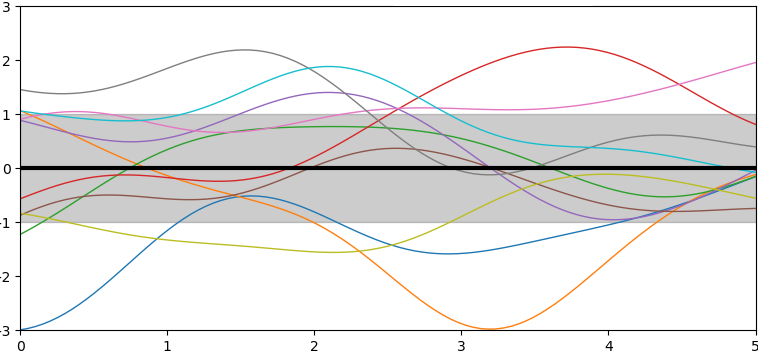
\includegraphics[width=0.45\textwidth]{RBF_prior}} 
		\hfill % no empty line here to avoid staring a new paragraph (figures will be vertically aligned)
		\subfigure
		[RBF kernel posterior ($length scale = 0.279$)]
		{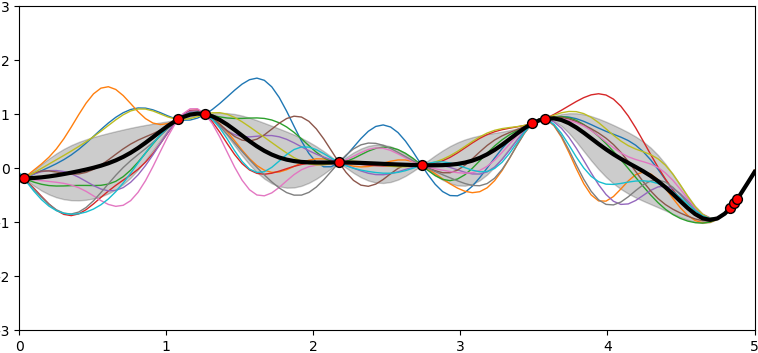
\includegraphics[width=0.45\textwidth]{RBF_posterior}}
		\caption
		[Prior and posterior of RBF kernel]
		{Prior and posterior of RBF kernel.
			This kernel typically results in smoothed functions.
			The length scale parameter determines the length of the \enquote*{wiggles} of the functions}
		\label{fig:RBF_prior_posterior}
	\end{figure}
	
%	\item[Rational quadratic kernel]
%	This kernel can be seen as a scale mixture (infinite sum) of RBF kernels with different length scales.
%	Therefore, \acp{gp} priors with this kernel expect to see functions which vary smoothly across many length scales.
%	It has two parameters: length scale $l > 0$ and scale mixture $\alpha > 0$.
%	The parameter $\alpha$ determines the relative weighting of large-scale and small-scale variations.
%	When $\alpha$ $\lim$ $\inf$, the RQ kernel is identical to the SE kernel, as described by
%	
%	\begin{equation}
%		\label{eq:RQ_kernel}
%		k_{RQ}(\{\sigma, \alpha, \ell\}, x, x') = \sigma^2 \left( 1 + \frac{\lVert x_1 - x_2 \lVert ^2}{2\alpha \ell^2} \right)^{-\alpha}.
%	\end{equation}
%	\eqname{Rational quadratic kernel}
\end{description}

\todo[inline]{here write about the initial parameter values, boundaries, etc.}

\section{Interpolating data using kriging}
\label{sec:interploating_data_using_kriging}

\todo[inline]{explain that we use GP to obtain ``missing'' data points in the feature vectors of the speakers to make the time series parallel and comparable.}

\citet{Galvez2020unifiying}\\ % compare to the rather simplistic (and naive) approach taken here (based on TAMA)
\citet{Kousidis2008towards}\\ % original TAMA paper. read again, but seems like it's glorified moving average. say that my appraoch actually learns the curve of the speaker and doesn't just interpolate, which allows continuous predictions and more evolve description.
\citet{Kousidis2009monitoring}\\ % another TAMA paper, with an a bit more concrete example

\todo[inline]{as an introduction, present Kriging, use this for a start \url{https://en.wikipedia.org/wiki/Kriging}}
\todo[inline]{definitely write down and explain the kernel we used for interpolation (probably a sum kernel of product kernel)}
\todo[inline]{don't forget to mention the log maximum likelihood of the interpolation}
